\begin{pagefigure}
\checkoddpage \ifoddpage \forcerectofloat \else \forceversofloat \fi
\centering

    \begin{subfigure}[t]{0.5435\textwidth}
        \centering
        \includegraphics[width=\linewidth]{"images/2016/other-finds-2016/kenneth-eyrie__2_".jpg} 
        \caption{} \label{moon door}
    \end{subfigure}
        \hfill
\begin{subfigure}[t]{0.4465\textwidth}
\centering
\includegraphics[width=\linewidth]{"images/2016/other-finds-2016/kenneth-book".jpg}
 \caption{}\label{reading in the bivi}
\end{subfigure}
    \vspace{0cm}
    \begin{subfigure}[t]{\textwidth}
    \centering
        \includegraphics[width=\linewidth]{"images/2016/other-finds-2016/kenneth-hammer".jpg} 
        \caption{} \label{hammer in B9}
    \end{subfigure}
    \caption{
    \emph{(a)}  Kenneth Tan, preparing to abseil through the lower entrance of \protect\passage{B9} - \protect\passage{Jackie's blower} - \protect\passage{the Eyrie}. Below a spur of rock underneath which the \protect\passage[entrance]{Monatip} entrance was first spotted \pic{Rhys Tyers}
     \emph{(b)} Mountain life can also be about relaxing in the bivi, reading, cooking or taking up a new hobby.
     \emph{(c)}  Kenneth Tan in the process of bolting a small pitch in \protect\passage{B9} cave, the way on was another too tight rift \pic{Arun Paul}}
\end{pagefigure}
\clearpage

\section{Additional findings around Migovec}

\subsection{The Auld Alliance}
William French and William Scott embarked on a journey to the \passage{Monatip}-\passage{NCB} connection passages, intent on dropping a rope down one of the several ongoing leads in the `\passage[|see{Vsporedni Svet}]{Avenue of Pitches}'. They entered via M2 to reach the \passage{NCB} section of the cave and, navigating their way from boulder choke to boulder choke entered the continuation of the horizontal passage. Although they had rope and bolts, they only managed to reach a ledge 15m down on a large pitch, reported to be going big. This pitch is located  about 100m to the south west old system's \passage{Level 2}, whose large piercing shafts had required many infamous traverses to overcome; therefore it remains a tantalising lead for exploration.





\begin{marginfigure}
\checkoddpage \ifoddpage \forcerectofloat \else \forceversofloat \fi
\centering
 \includegraphics[width=\linewidth]{"images/2016/other-finds-2016/will_scott_sunset".jpg} 
 \caption{Spirits lifted whilst admiring an unlikely sunset after a miserable rainy day in the Bivi \pic{Tanguy Racine}}
 \label{Sunset}
\end{marginfigure}



\subsection{The Stile, Cattlegrid}
Early on the expedition, Rhys Tyers noted a couple of muddy crawls leading off the bottom of \passage{Knot Very Good} pitch. Over the course of several trips, the \passage{Cattlegrid} passage was explored to a wet 10m pitch and a small maze of low phreatic crawl-ways connected to \passage{Smer0} via \passage{The Stile}. The tubes had been rejuvenated by two vadose steams whose stepped descent provided a relatively easy access to the pushing front. After a couple of visits however, the mud which had lain undisturbed for tens of thousands of years in neat little alcoves was liberally plastered over white walls.

\subsection{B9 - Jackie's blower revisited (aka the Eyrie)}
Arun Paul chanced upon the large entrance of \passage{B9} near the Western edge of the \passage{Plateau}, and almost due west of the Bivi. Discovered in 1994 and revisited on a number of occasions since, the cave provided a gentle introduction to expedition caving. Rhys Tyers led a bolting trip there to push the bottom pitch, as well as rig the `Moon Door' a rift heading out of the cliff face and providing a airy view of the \passage[valley]{Tolminka} valley below.

 \subsection{A hike to the sources of the Tolminka}
 About halfway during the expedition, I thought I'd like a shower, thank you very much. Successfully ensnared most of the novices with me (Kenneth, Arun and Will Scott): we went down to \passage{Kal} early in the morning to help with some of the repairs at the middle hut, but it turned out Fratnik, Maffi and Tja\v{s}a had already done most of the work, so we only had a quick coffee and \v{z}ganje before going to \passage{Tolmin} proper for a well deserved pizza and a couple of beers. 
 
 The morning after Will and I walked up to \v{C}ardg, along the path to \passage{Planina Polog}. The sun was out, the heat rising from the bottom of the valley with the rush of the \passage{Tolminka}. We arrived at the springs: a massive scree cone coming from \passage{Krn} dammed by a curved brick wall: very impressive! 
 
There were two flights of limestone walls rising up towards \passage{Kuk} and \passage{Mig}: I took photographs from our viewpoint and then looked at the skyes: dark, ominous clouds were obscuring the sun. Opting to walk back briskly, we only managed to reach the 'Welcome to Triglav National Park' sign before heavens opened completely. 

Under this heavy rain, we trudged along the valley bottom gravel road, twisting and turning towards the Tolmin gorges, and finally, popping out slightly above Zatolmin. Back at Tetley's flat, I looked at some of our pictures and noticed, zooming in, that I could make out the entrance to Primadona, and that rock bridge Fratnik had mentioned. If only we'd had it at the beginning, it would have saved a couple of days fruitless efforts! 
 
 \begin{figure*}[t!]

 \begin{subfigure}{0.70\textwidth}
\frame{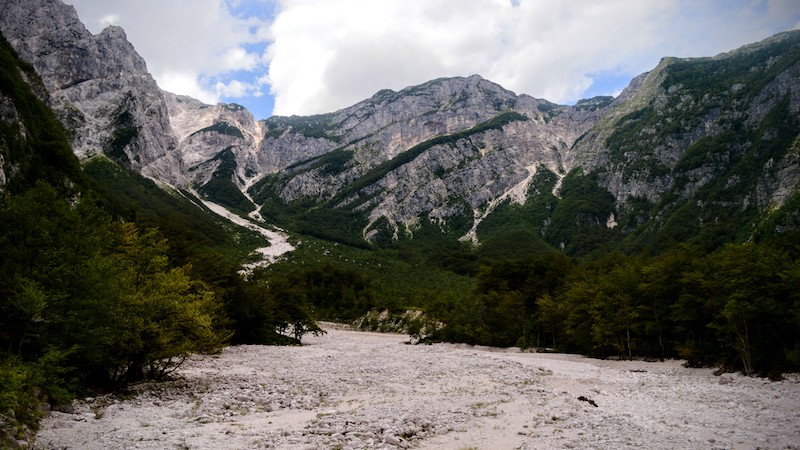
\includegraphics[width = \textwidth]{images/2016/other-finds-2016/izvhir_tolminka.jpg}}
\end{subfigure}
\hspace{3pt}
 \begin{subfigure}{0.29\textwidth}
\frame{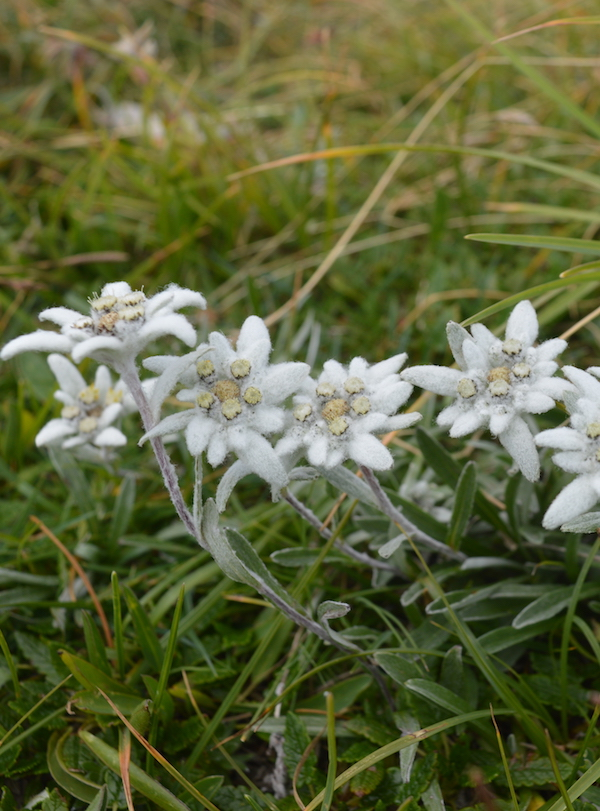
\includegraphics[width = \textwidth]{images/2016/other-finds-2016/edelweiss.jpg}}
\end{subfigure}
\caption{In the forest near the \protect\passage{Izvhir Tolminke}} \label{fig:izvhir tolminke}
 \end{figure*}
 
 \name{Tanguy Racine} 
\clearpage

\begin{pagefigure}
\checkoddpage \ifoddpage \forcerectofloat \else \forceversofloat \fi
\centering
\frame{\includegraphics[width=\textwidth]{"images/2016/other-finds-2016/end_of_expo".jpg}}
\caption{The expedition team relaxes for a drink and cottage cheese cake at \passage{Ravne}, thanks to the hospitality of the Koblucar family: Slavica, Zoran and Nada \pic{Tanguy Racine}}
\label{End of the expedition}
\end{pagefigure}

 \numbertable{
    \begin{tabular}{lrrrr}
    Sector & \multicolumn{1}{l}{\textbf{Passage name}} & \textbf{Survey length (m)} & \textbf{Stations} & \textbf{Average leg (m)} \\ \midrule
    \multirow{2}[0]{*}{Alkatraz} & \multicolumn{1}{l}{The Rock} & 129.35 & 28    & 4.79 \\
          & \multicolumn{1}{l}{Memory Lane} & \_    & 16    & \_ \\ \midrule
    \multirow{5}[0]{*}{Galerija} & \multicolumn{1}{l}{Cattle Grid} & 87.40 & 24    & 3.80 \\
          & \multicolumn{1}{l}{Galeria resurvey} & \_    & 10    & \_ \\
          & \multicolumn{1}{l}{Quantum State} & 70.40 & 15    & 5.03 \\
          & \multicolumn{1}{l}{Terminus} & 51.29 & 16    & 3.42 \\
          & \multicolumn{1}{l}{The Stile} & 65.38 & 19    & 3.63 \\ \midrule
    \multirow{8}[0]{*}{Karstaway} & \multicolumn{1}{l}{Colony} & 83.82 & 10    & 9.31 \\
          & \multicolumn{1}{l}{Gambler's Ruin} & 40.51 & 10    & 4.50 \\
          & \multicolumn{1}{l}{Hall of the Mountain King} & 104.00 & 14    & 8.00 \\
          & \multicolumn{1}{l}{Karstaway} & 192.08 & 40    & 4.93 \\
          & \multicolumn{1}{l}{Mighty Fine Indeed} & 32.33 & 6     & 6.47 \\
          & \multicolumn{1}{l}{Tight and Scrotty} & 43.79 & 10    & 4.87 \\
          & \multicolumn{1}{l}{Upside Down Chamber} & 119.11 & 12    & 10.83 \\
          & \multicolumn{1}{l}{What a Coincidence} & 221.33 & 31    & 7.38 \\ \midrule
    \multirow{2}[0]{*}{Monatip} & \multicolumn{1}{l}{Auld Alliance} & 34.16 & 7     & 5.69 \\
          & \multicolumn{1}{l}{Cloaca Maxima} & 335.61 & 54    & 6.33 \\ \midrule
    TTT   & \multicolumn{1}{l}{Déjà Vu} & 90.69 & 13    & 7.56 \\ \midrule
          &       &       &       &  \\
    \textbf{Total} &       & \textbf{1701.25} &       &  \\
    \end{tabular}}

\begin{pagesurvey}
\centering
\frame{\includegraphics[height=\textheight]{"images/2016/other-finds-2016/2016plan".pdf}}
\caption{2016 Plan Survey}
\label{}
\end{pagesurvey}

\begin{pagesurvey}
\centering
\frame{\includegraphics[height=\textheight]{"images/2016/other-finds-2016/ee2016".pdf}}
\caption{2016 Extended Elevation}
\label{}
\end{pagesurvey}
